\chapter{Method development}
\label{chap:md}

\section{Hemolymph sampling technique}
To minimize the possibility of contaminating hemolymph samples during extraction, a simple and time-effective sampling technique slightly modified from the nonlethal technique of Gustafson et al., 2005 was used. "Blind" methods of withdrawal through a notch in the posterior dorsal shell or through the exhalant syphon frequently resulted in considerable contamination with debris from the pallial fluid. Therefore, the hemolymph sampling technique employed was centered around achieving good visual contact with the posterior adductor muscle and the position of the needle within the muscle during hemolymph withdrawal, and was mainly constricted by the requirement of an intact digestive gland.

The digestive gland is located dorsally (towards the hinge), slightly off-center towards the anterior end of the shell (Eggermont, 2020). In order to access and see the posterior adductor muscle while staying clear of the digestive gland, the valves were prised apart ventrally by gently forcing a tissue forceps between the valves midway of the mussel's length, or slightly posterior of the byssal mass (Fig. \ref{fig:Hemolymph_sampling_illustration}a). When the pallial cavity opened, pallial fluid (seawater) was drained away from the posterior adductor muscle by positioning the mussel's umbo on a paper tissue for 15-30 seconds. Since the posterior adductor muscle is oblong in the anteroposterior direction, penetrating the muscle from the posterior end pointing straight anteriorly gave the operator better margins to avoid piercing the muscle.

To create a free path to the muscle from the posterior direction, the connecting mantle immediately surrounding the exhalant syphon where cut with a scalpel (Fig. \ref{fig:Hemolymph_sampling_illustration}b and d), holding the blunt spine of the scalpel blade facing the posterior adductor muscle. Thus, when illuminating the pallial cavity from above with the ventral aspect facing upwards, the operator was able to supervise the position of the needle inside the posterior adductor muscle sinus through the slightly transparent muscle fibers, as seen in Fig. \ref{fig:Hemolymph_sampling_illustration}c.

For this work, 1.0 mL syringes equipped with sterile 23 gauge hypodermic needles were used. Hemolymph samples were gently withdrawn at an approximate rate of 1.0 mL/min, in order to prevent the negative pressure inside the muscle from drawing in pallial fluid between the muscle fibers. The mussels were placed in the palm of the operator's non-dominant arm, 3$^{rd}$-5$^{th}$ digits firmly gripping the mussel, first and second digits holding the syringe steady in the anteroposterior direction, while the dominant arm were used to withdraw the syringe plunger.

\begin{figure}[t]
    \centering
    \begin{subfigure}[b]{.45\textwidth}
        \centering
        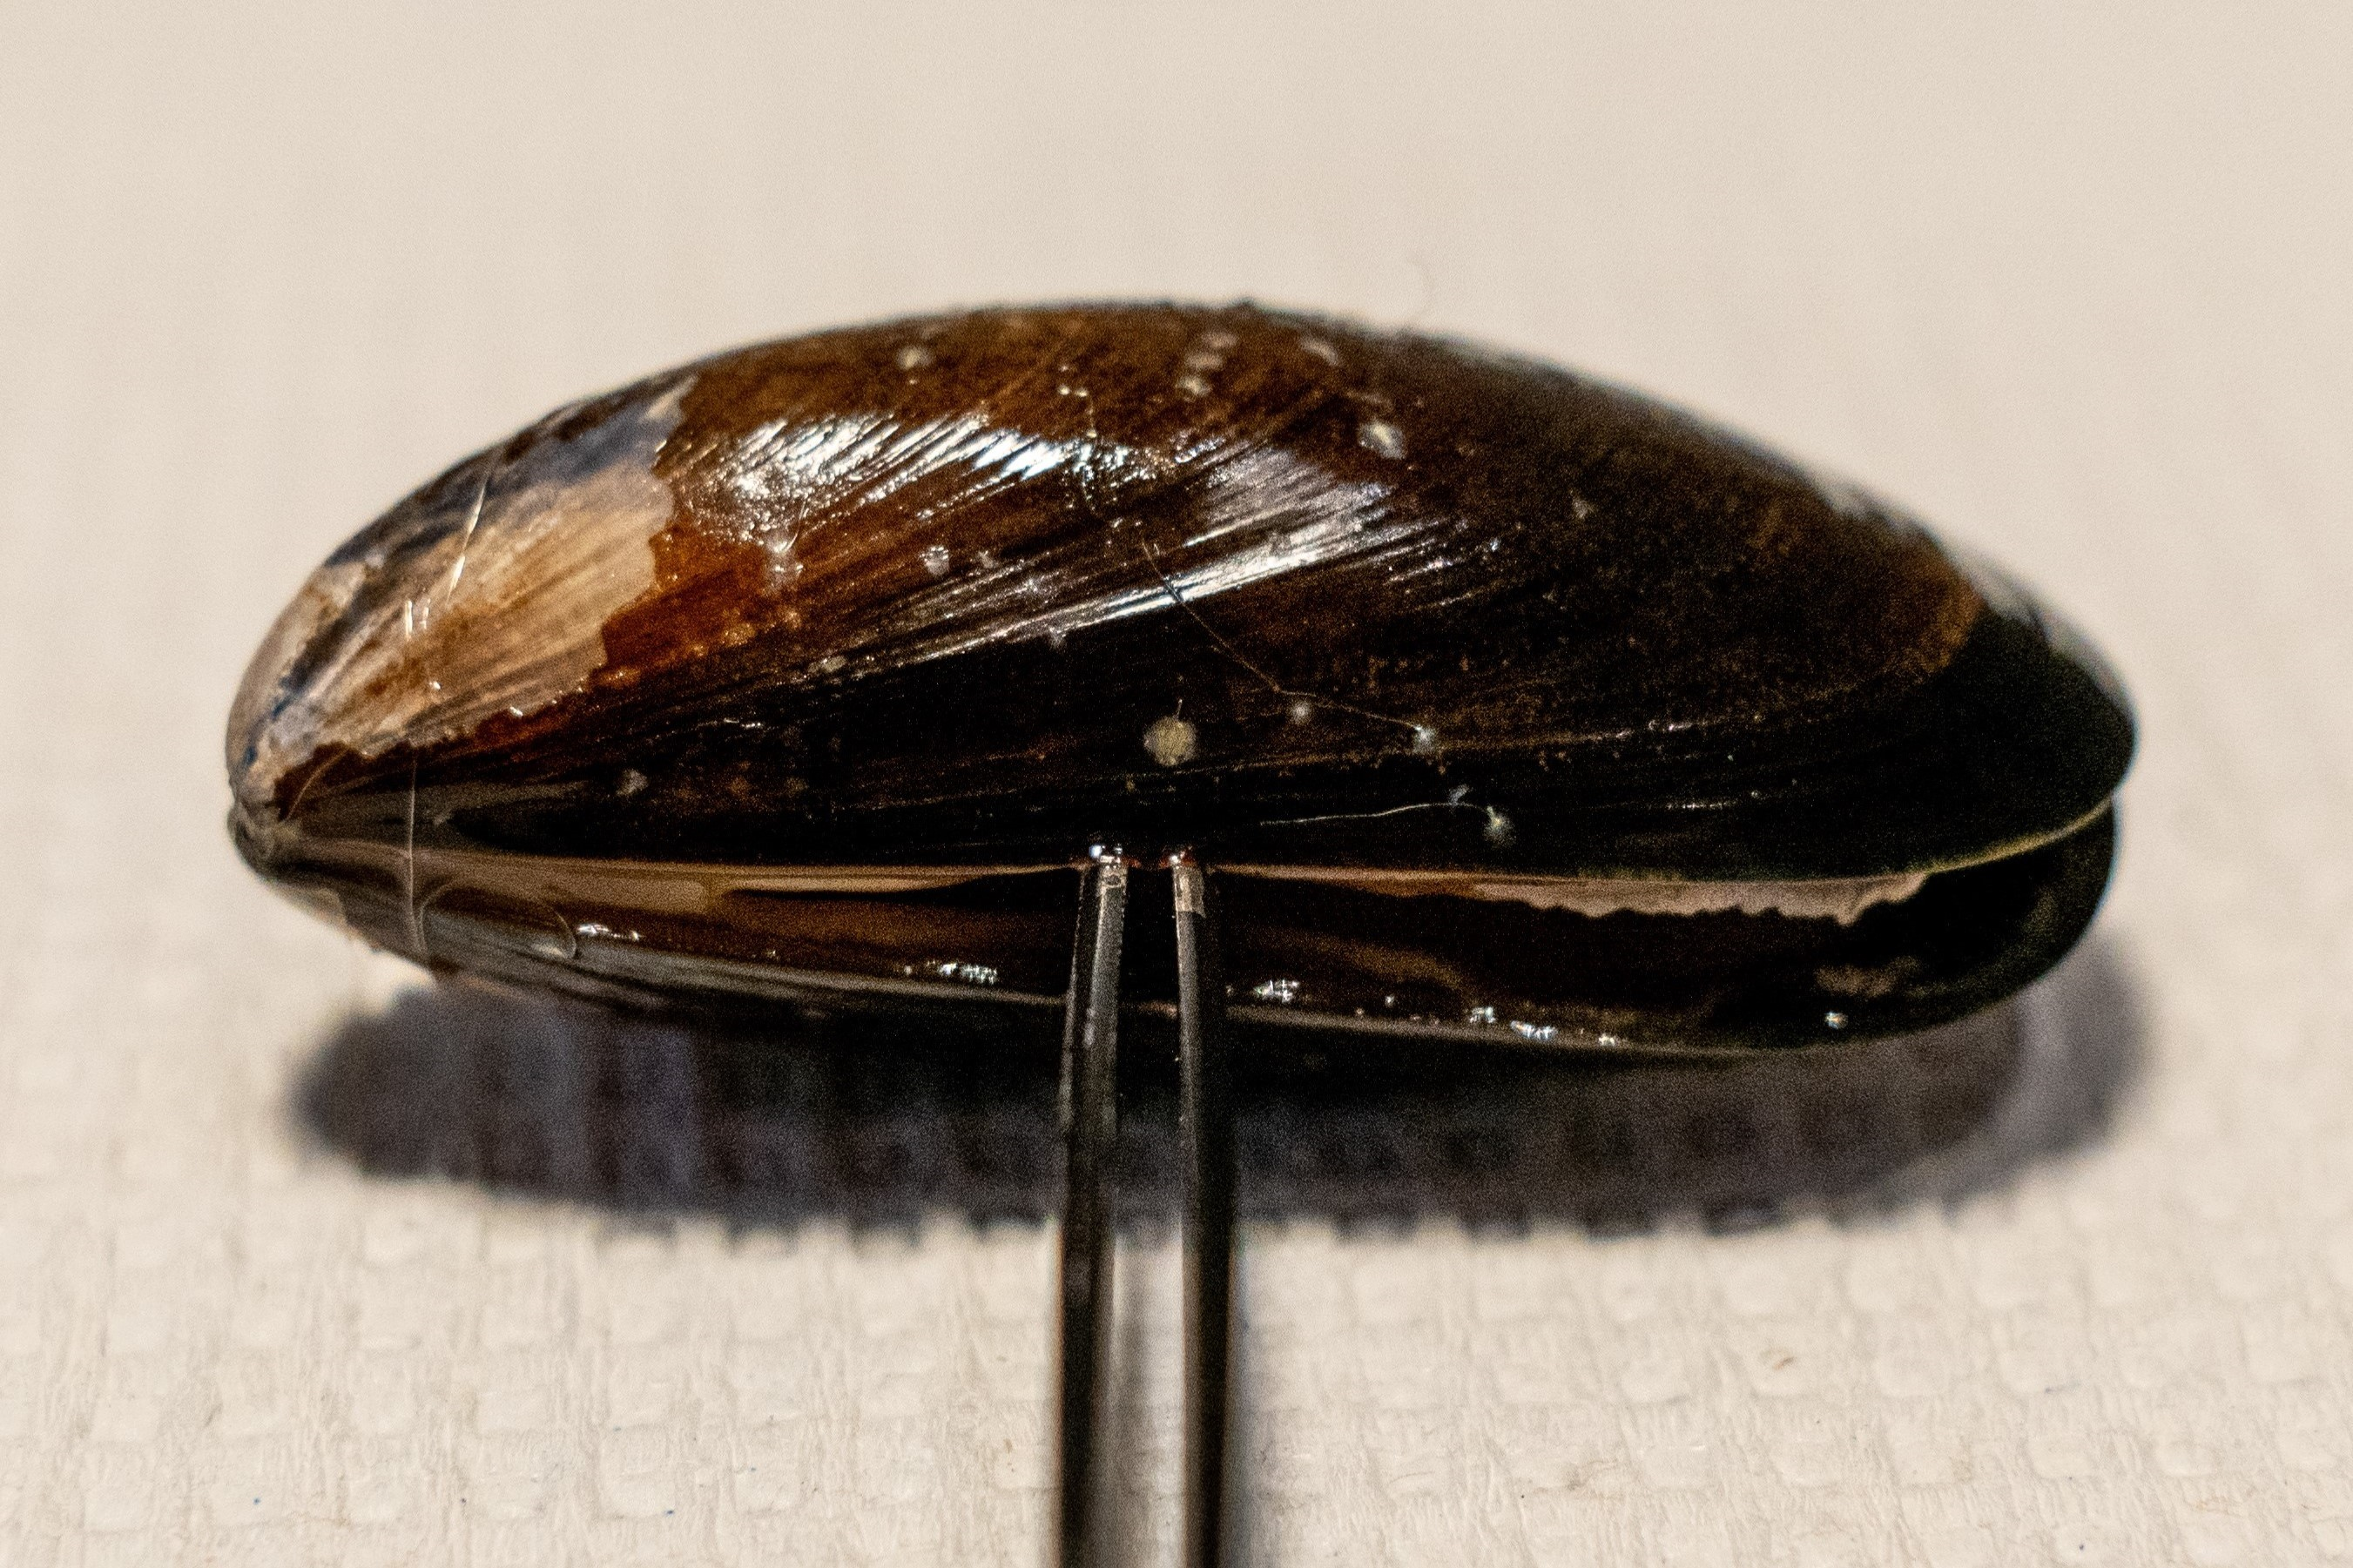
\includegraphics[width=\textwidth]{figures/Sampling technique/forceps square color.jpg}
        \caption{Placement of forceps between valves on the ventral side of the mussel.}
        \label{sfig:a}
    \end{subfigure}
    \hfill
    \begin{subfigure}[b]{.45\textwidth}
        \centering
        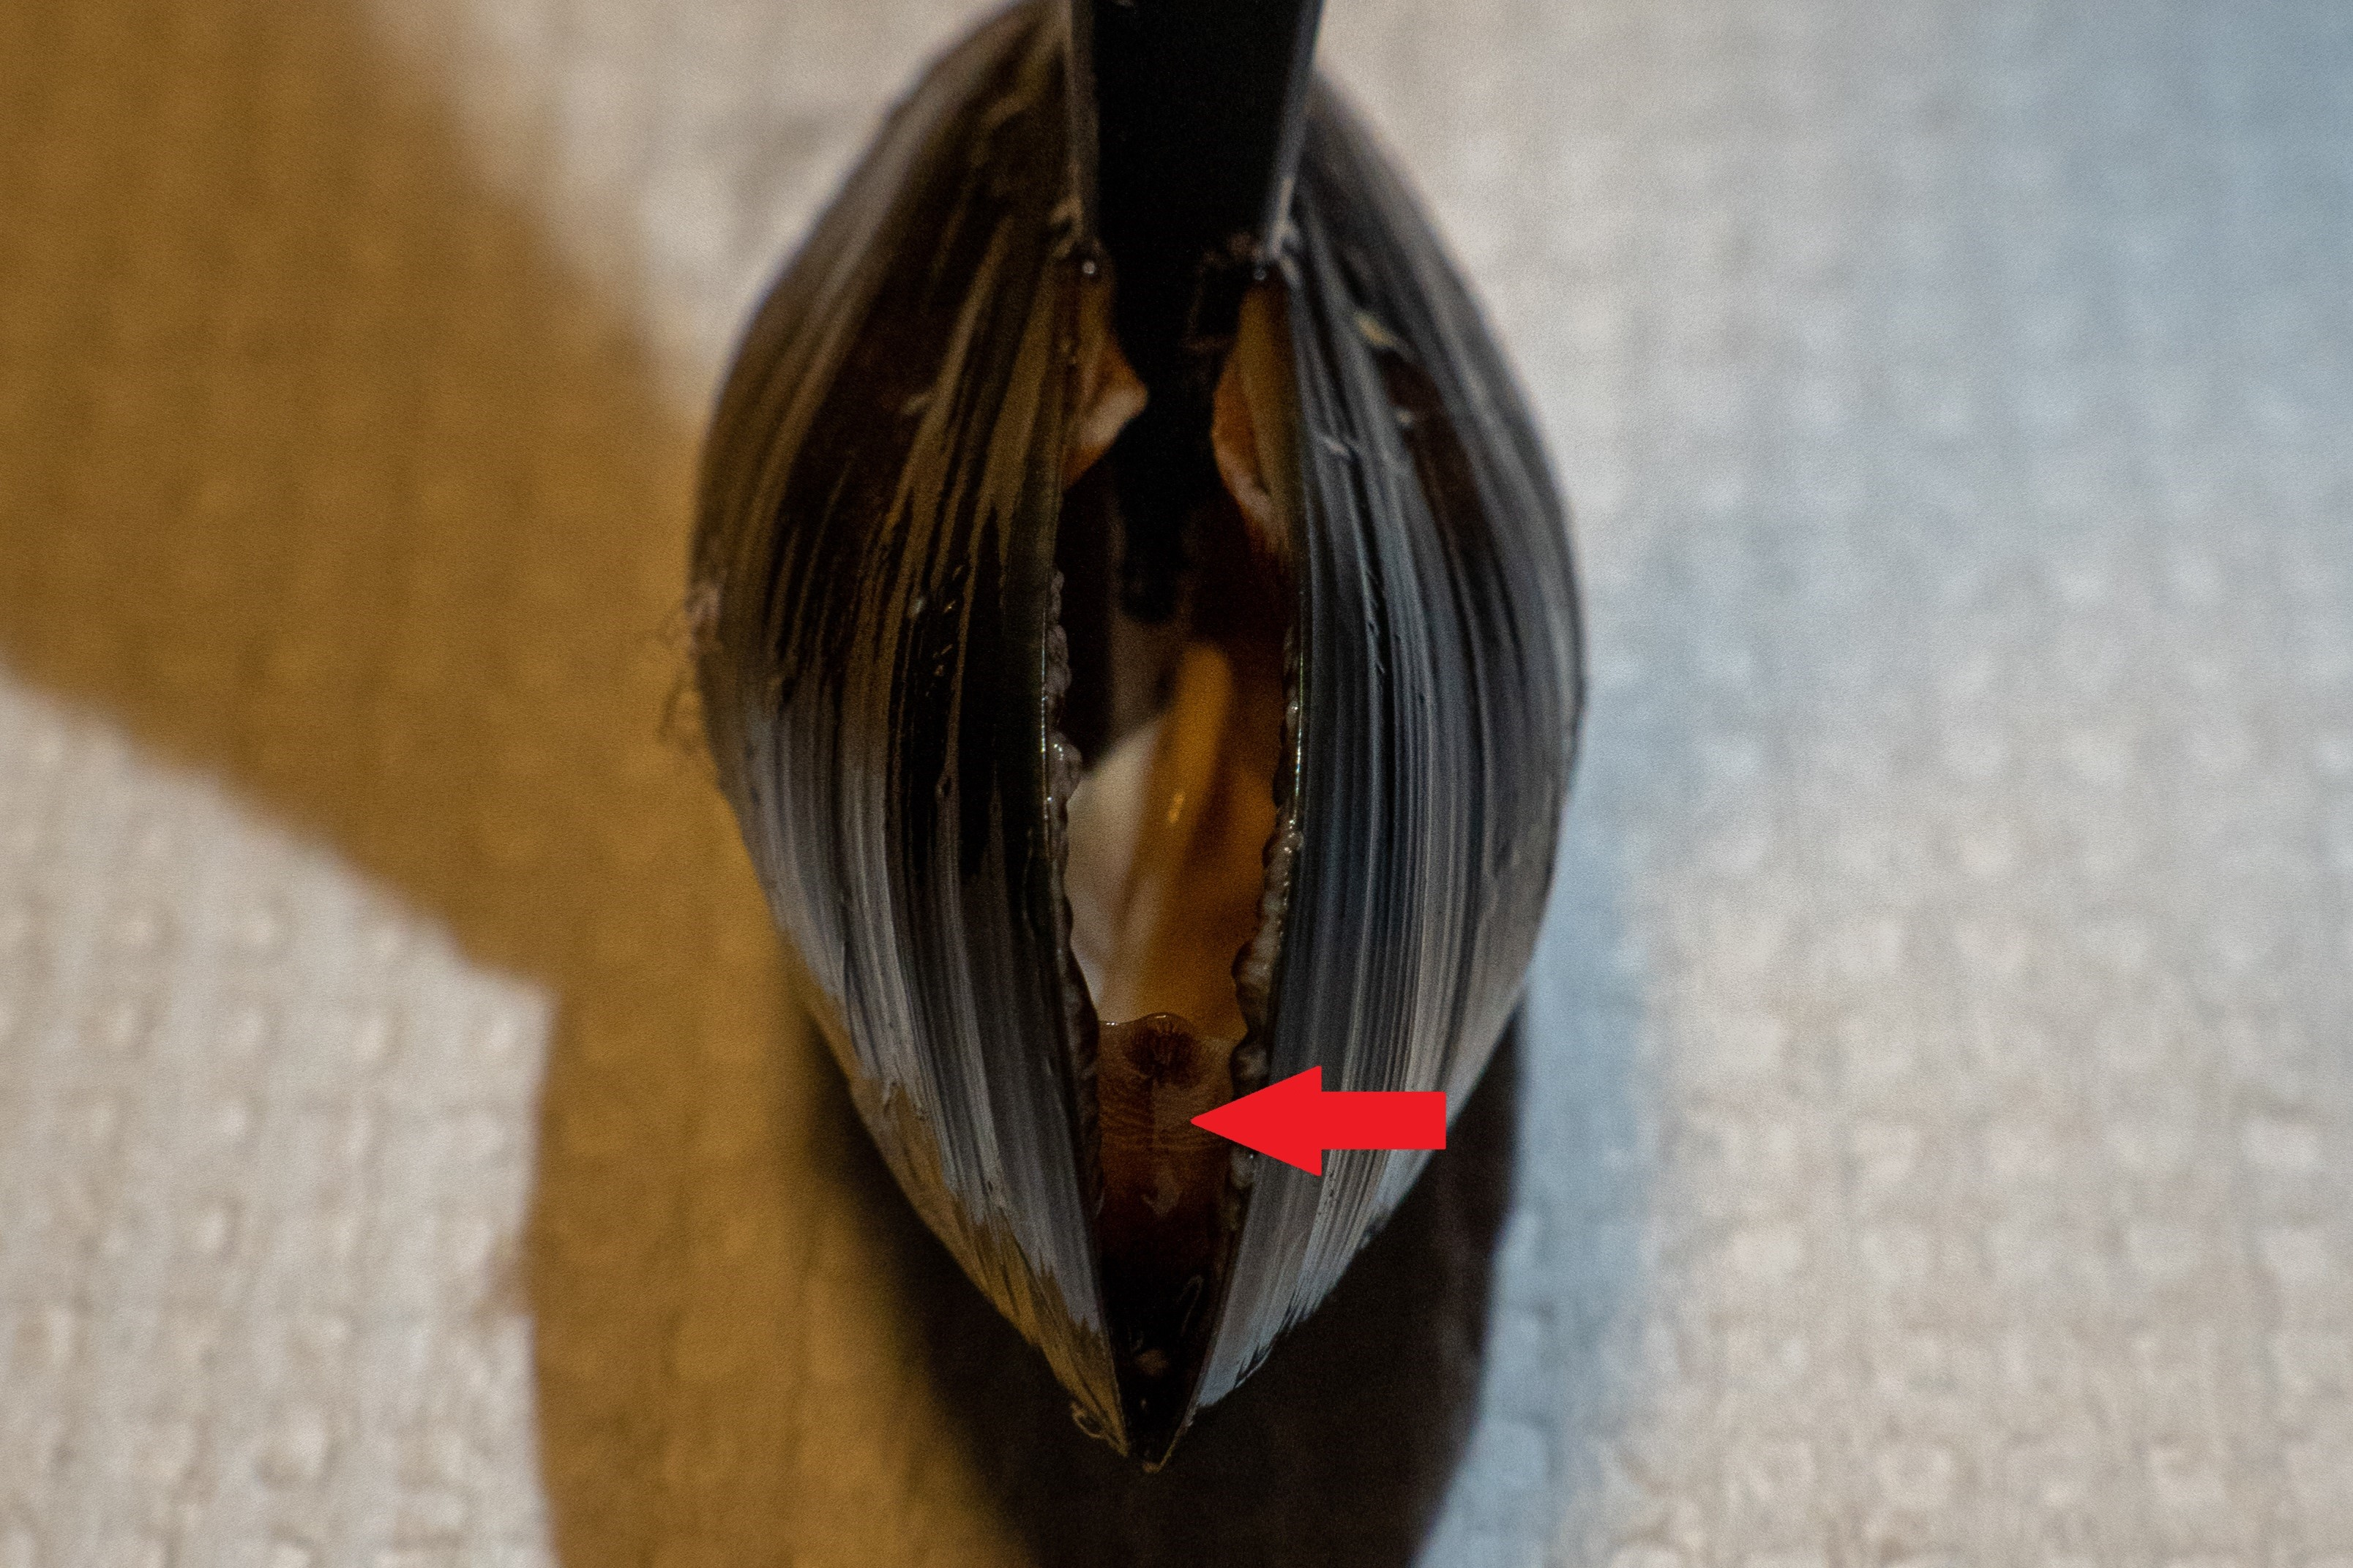
\includegraphics[width=\textwidth]{figures/Sampling technique/uncut color 3495.jpg}
        \caption{Posterior aspect of mussel with the connecting mantle (red arrow) intact.}
        \label{sfig:b}
    \end{subfigure}
    \newline
    \begin{subfigure}[b]{.45\textwidth}
        \centering
        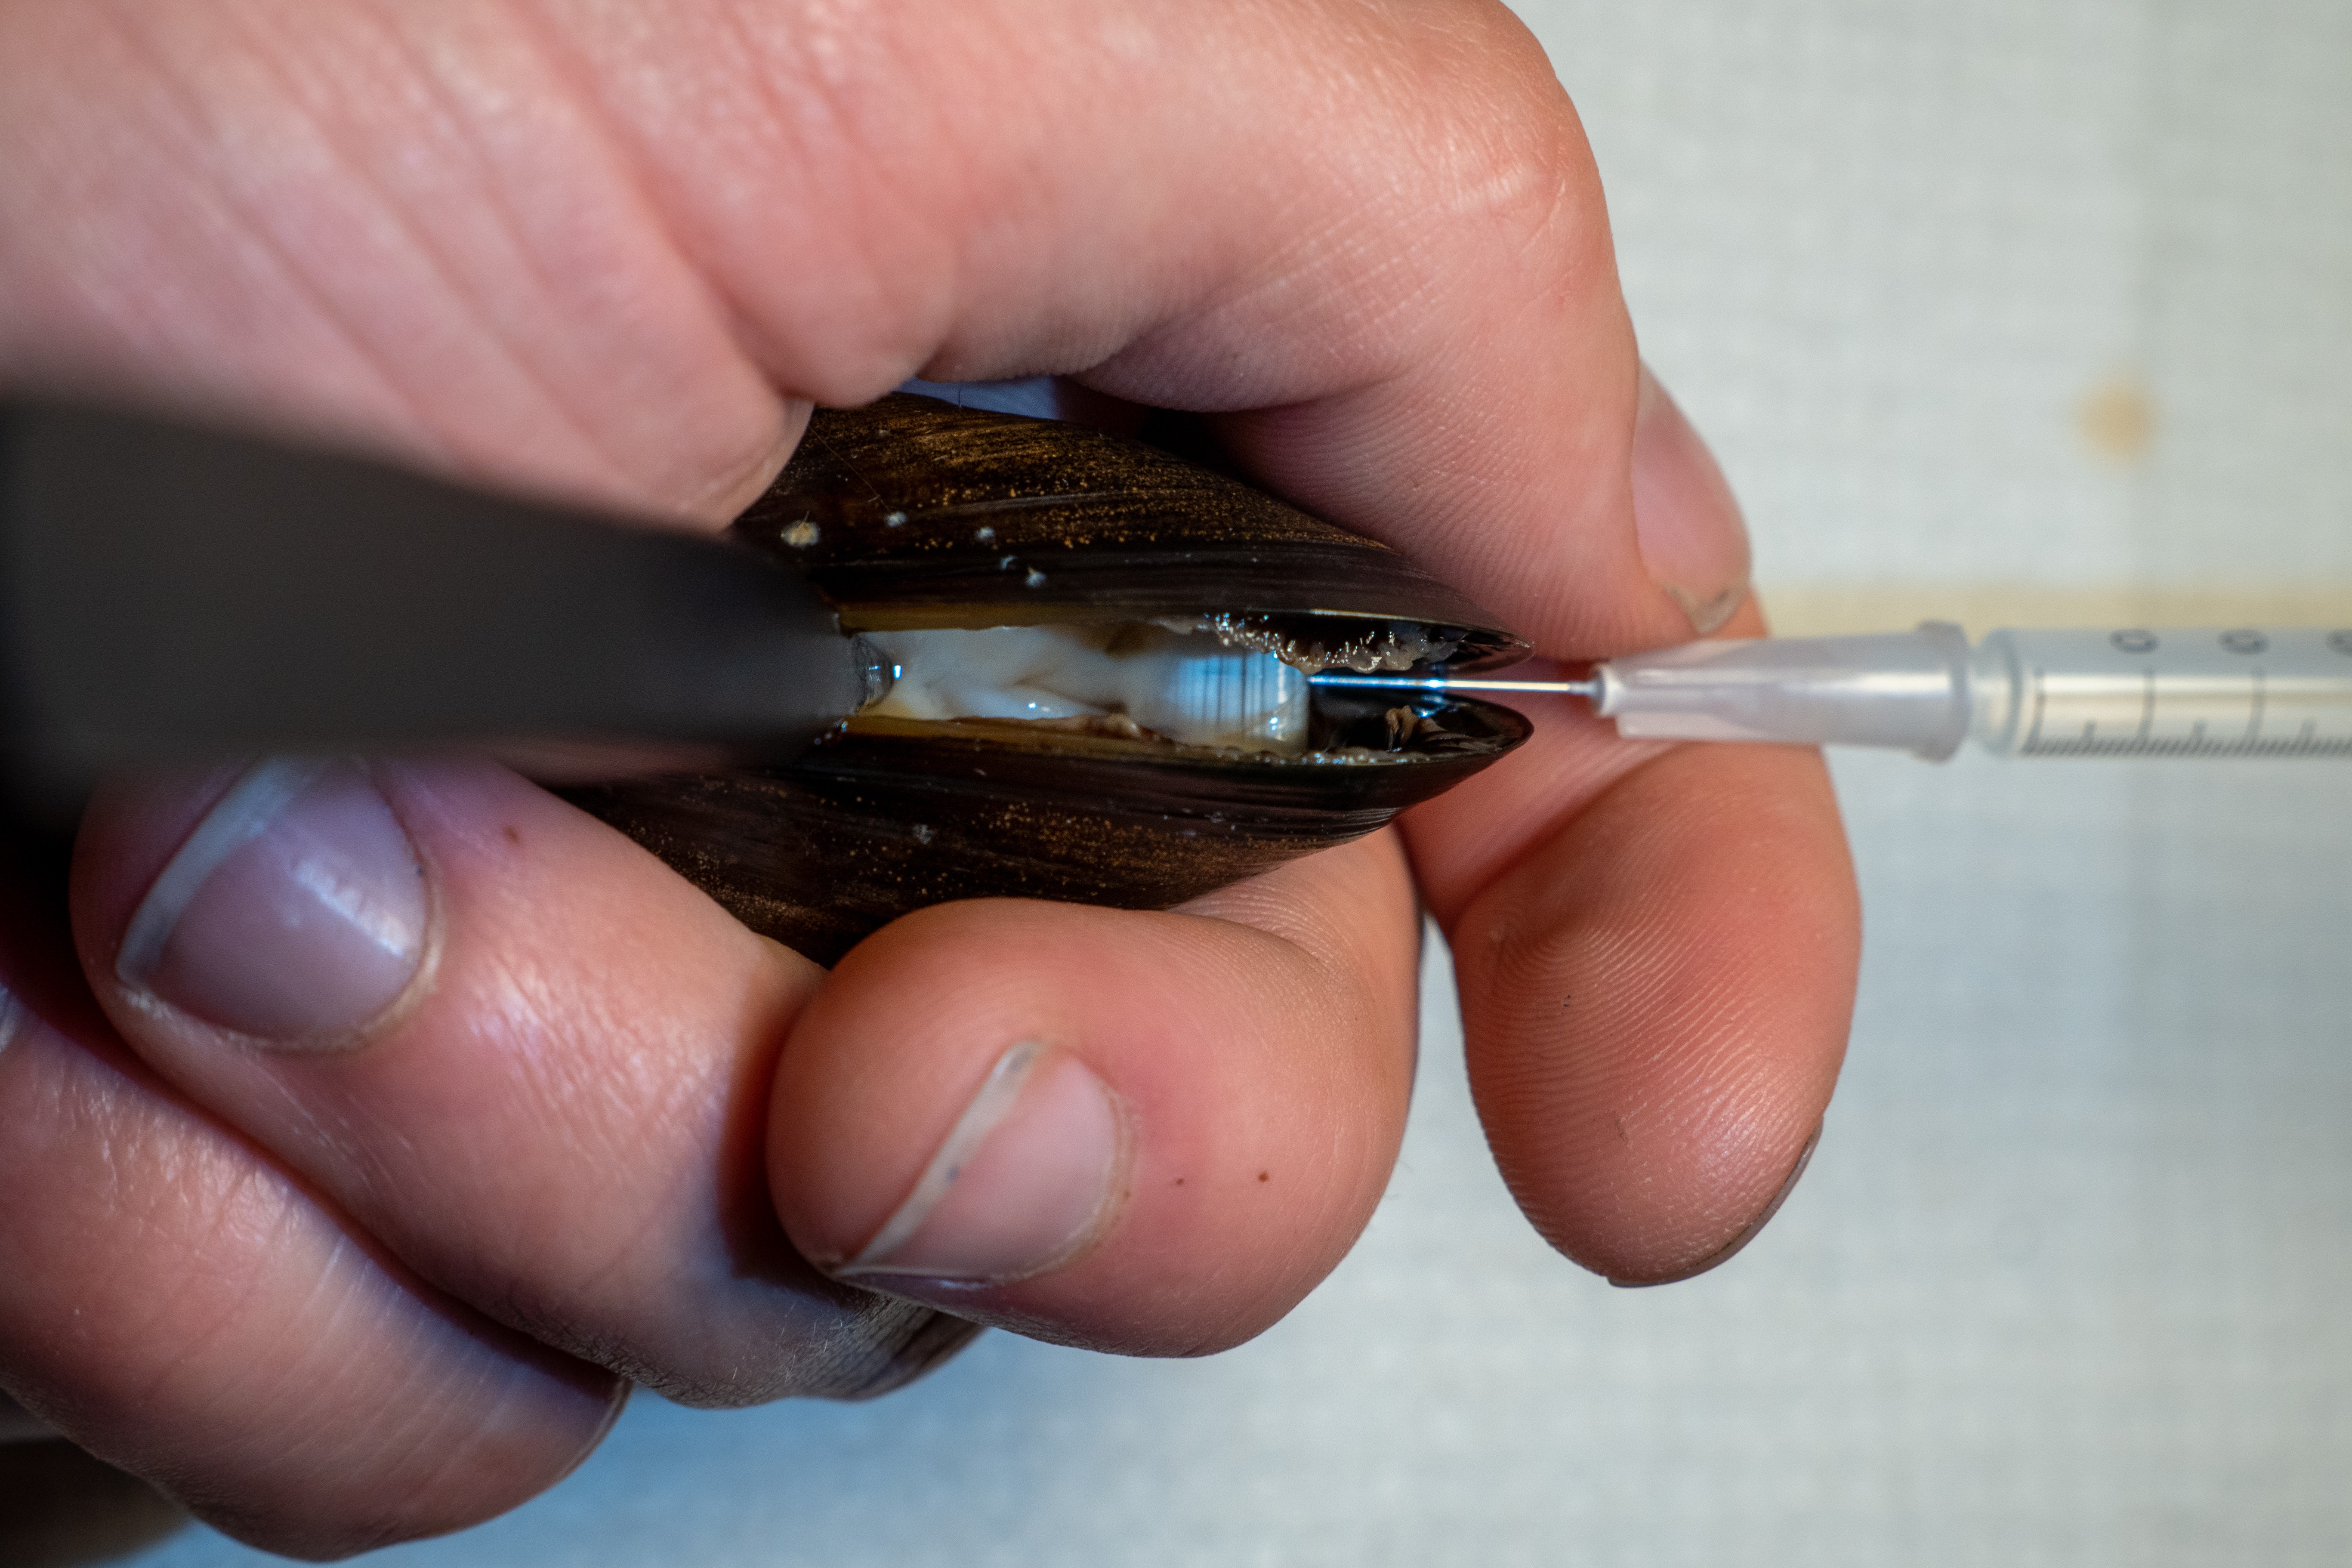
\includegraphics[width=\textwidth]{figures/Sampling technique/hands colors centered.jpg}
        \caption{The mussel grip and needle alignment employed, seen from the operators perspective. }
        \label{sfig:c}
    \end{subfigure}
    \hfill
    \begin{subfigure}[b]{.45\textwidth}
        \centering
        \includegraphics[width=\textwidth]{figures/Sampling technique/possible match.jpg}
        \caption{Mussel with visible posterior adductor muscle (red arrow) where the mantel was cut.}
        \label{sfig:d}
    \end{subfigure}
    \caption{An illustration of the method employed to extract hemolymph from M. edulis in order to avoid off-target withdrawal of fluid from the lungs or remaining pallial fluid. The pictures were taken using a Sony A6400 mirrorless digital camera with a Tamron 17-70mm F/2.8 lens, and edited with Adobe\textsuperscript{\textregistered} Lightroom Classic 12.0 image editing software.}
    \label{fig:Hemolymph_sampling_illustration}
\end{figure}

\section{Selection of hemocyte medium}
The hemocytes of \emph{M. edulis} have a tendency to form aggregates upon mechanical stress, e.g. when the hemolymph is withdrawn through a thin syringe needle. Since accurate flow cytometric analyses rely on single-cell measurements, there was a need to minimize hemocyte aggregation during staining procedures, until the samples could by analyzed on the flow cytometer. For the purpose of scoring nuclear anomalies in stained hemolymph smears, it is also essential to keep the hemocytes from clumping together. The basophilic hemocytes have a tendency to spread on top of each other, rendering their individual cytoplasms indistinguishable from one another.

In the literature, several authors have dealt with this challenge by aspirating hemolymph samples directly into slightly acidic EDTA-containing solutions buffered by citric acid (\cite{Söderhall1983, Bachere1988, LeFoll2010}). Since hemocyte aggregation is a Ca$^{2+}$-dependent process (\cite{Torreilles1999, Chen1995}), withdrawal of hemolymph into buffers containing divalent metal-ion chelators effectively slows the rate of hemocyte aggregation, allthough it does not inhibit aggregation completely (\cite{Chen1995}). Another frequently reported method is to dilute the hemolymph in cold filtered seawater (FSW), while keeping the samples on ice prior to analysis. 

In search for the most effective method for this work, hemolymph samples were withdrawn into syringes pre-filled with a number of different "anticoagulant" or "antiaggregative" buffers (1:1) reported in the literature. The degree of aggregation was initially evaluated by inspecting hemolymph smears prepared following the method of \cite{Bolognesi2012} under 10x magnification. After preliminary testing, the most promising buffers encountered where the Modified Alsever's Solution (MAS, pH=6.2), and the similar Anticoagulant Buffer (ACB, pH=7.6) with EDTA reported by \cite{Pipe1997}. Since the use of EDTA (MAS and ACB), acidic pH (MAS) or keeping samples on ice (FSW) might introduce inconveniences related to staining procedures, extra handling requirements and possibly impairing hemocyte viability, two experiments were devised in order to test their relative effects on hemocyte aggregation and viability - under the conditions intended for our flow cytometric analysis. Thereby, a cost-effect assessment could be carried out to arrive at the most suitable buffer for this work.

\subsection{Hemocyte aggregation}
An experiment was seeded from the observation that FCM singlet hemocyte counts tended to decrease over time from hemolymph withdrawal, and were based on the assumption that aggregation was the main driving factor. The proportion of aggregated hemocytes in a sample at a given time could therefore be retraced from the initial hemocyte count when performing several counts of the same sample over time. Since the difference in density between buffers would be negligible, the sedimentation rates of free hemocytes would be equal in all three groups. Any observed differences would thus be caused by differences in the buffers' ability to inhibit aggregation.

500 \micro L hemolymph was withdrawn from 23 individual mussels into syringes prefilled with either 500 \micro L MAS (RT, n=7), ACB (RT, n=8) or cold Hemolymph Saline (MPSS, \SI{4}{\celsius}, n=8). Tris-buffered MPSS (pH=7.4) was used as a proxy for FSW, such that pH and osmolarity could be controlled. The diluted hemolymph was transferred to 12$\times$75 mm polystyrene tubes and the initial hemocyte count were determined by acquiring 20 \micro L sample on the flow cytometer immediately thereafter. Each sample was run with identical acquisition and fluidics settings (see table \ref{tb:FCM_settings}), and the cells were gated on by a singlet inclusion gate (FSC-A vs. FSC-H) and a hemocyte gate (FSC-A v. SSC-A, see gating strategy). To account for any extra aggregation occurring from gentle mixing with flow cytometry reagents in the planned assay, each sample was gently pipetted up and down four times following the initial count. The second count were performed precisely 15 minutes later to mimic the incubation periods of our flow cytometry reagents. Three more singlet hemocyte counts where acquired from each sample at 30, 45 and 60 minutes post-withdrawal, to discern the buffers' ability to prevent aggregation during longer incubation periods. Samples withdrawn into MPSS were kept on ice between each singlet hemocyte count.

The proportion of aggregated hemocytes where calculated according to equation \ref{eq: proportion_agg}.

\begin{equation}
    \label{eq: proportion_agg}
    \hat{p} = \dfrac{N_{t0} - N_{tx}}{(N_{t0} - N_{tx}) + N_{tx}} = \dfrac{N_{t0} - N_{tx}}{N_{t0}}
\end{equation}

\begin{equation}
    \label{eq:agg_free_matrix}
    y = 
    \begin{pmatrix}
      N_{t0_{1}} - N_{tx_{1}} &  N_{t0_{1}} \\
      N_{t0_{2}} - N_{tx_{2}} &  N_{t0_{2}} \\
      N_{t0_{3}} - N_{tx_{3}} &  N_{t0_{3}} \\
      \vdots                   & \vdots       \\
      N_{t0_{n}} - N_{tx_{n}} &  N_{t0_{n}} \\
    \end{pmatrix}
\end{equation}
\
Where $\hat{p}$ is the proportion of aggregated hemocytes, N$_{to}$ is the initial number of singlet hemocytes in the sample and N$_{tx}$ is the number of singlet hemocytes at time x after hemolymph withdrawal. The proportion of aggregated hemocytes were modelled as a function of log time, with buffer as a categorical explanatory variable, using the base R glm() function with a "quasibinomial" error distribution and "logit" link function, as shown in Code listing 3.1. Instead of using the calculated proportions ($\hat{p}$), the response variable was formatted as a two-column matrix of aggregated and singlet hemocyte counts (see equation \ref{eq:agg_free_matrix}), such that logistic regression was possible. The logistic GLM model coded the categorical explanatory variable's factor levels into dummy variables (see equation \ref{eq:dummy_variables}), and used the MAS buffer as reference level. The resultant logistic model can be written out as in equation \ref{eq:logit} on the original scale, where $\alpha + \beta_{1}x_{i}$ is the linear predictor of the reference level, $\alpha_{2}$ and $\alpha_{3}$ are the difference in y-intercept for the MPSS and ACB buffers, while $\beta_{2}$ and $\beta_{3}$ are the differences in slopes for the same buffers, respectively. The data is presented in figure \ref{fig:aggregation}, together with the three buffers' "sub-models".

\begin{lstlisting}[language=R, caption = {The R source code run to fit the logistic proportion aggregation model.}]
model = glm(y ~ log(t) + Buffer + log(t):Buffer,
family = quasibinomial(link = "logit")
\end{lstlisting}

\begin{equation}
    \label{eq:dummy_variables}
D_{2} =\begin{cases}
      1, & \text{MPSS}\\
      0, & \text{not MPSS},
    \end{cases}
    \quad
D_{3} =\begin{cases}
      1, & \text{ACB}\\
      0, & \text{not ACB}
    \end{cases}
\end{equation}

\begin{equation}
\label{eq:logit}
\hat{p}_{i} = \dfrac{1}{1 + e^{-(\alpha \: + \: \beta_{1} x_{i} \: + \: \alpha_{2} D_{2} \: + \: \alpha_{3} D_{3} \: + \: \beta_{2} D_{2} \: + \: \beta_{3} D_{3} \: + \: \epsilon_{i})}}
\end{equation}

\begin{figure}[!ht]
    \centering
    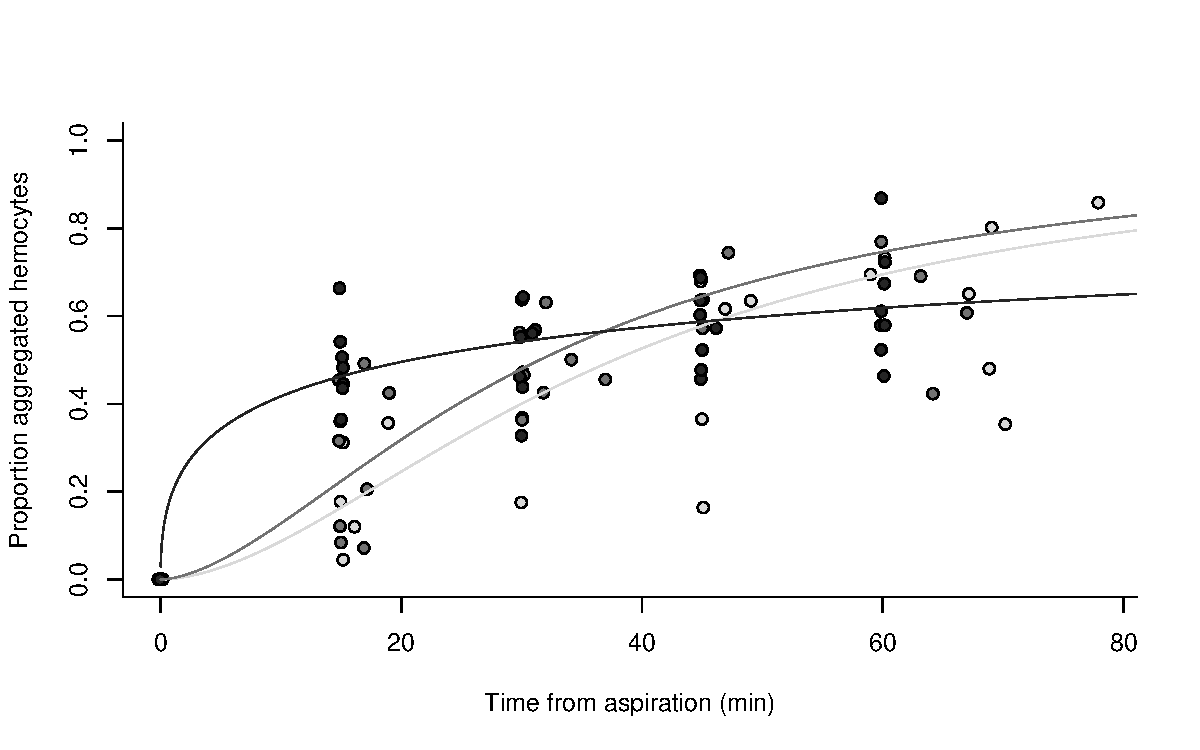
\includegraphics[width=1.0\textwidth]{figures/Method development/agg_plot_scaled.pdf}
    \caption{The proportion of aggregated hemocytes in 250 \micro L hemolymph withdrawn into an equal volume of Modified Alsever's Solution (\protect\lysegraacircle, n=7), Anticoagulant Buffer (\protect\graycircle, n=8) or Marine Physiological Saline Solution (\protect\darkgraycircle, n=8), plotted against time (min) after withdrawal from the posterior adductor muscle. The three regression lines illustrate the predicted proportions at time t for the three different buffers, as predicted by the fitted logistic regression model.}
    \label{fig:aggregation}
\end{figure}

Interpreting the logistic sub-models, it is evident that MAS and ACB effectively slowed the rate of aggregation during the first 30 minutes post-withdrawal. When MAS was used as hemocyte medium, the predicted mean proportion of aggregated hemocytes after 15 minutes was 0.16, CI = (0.12, 0.22). This was not significantly different from the predicted mean proportion when ACB was used (0.22, CI=(0.18, 0.28)), but both buffers containing EDTA and lacking free Ca$^{2+}$ were predicted to have significantly lower hemocyte aggregation after 20 minutes, compared to samples that were withdrawn into MPSS and kept on ice (0.46, CI=(0.33, 0.60)).

Although the model is over-dispersed, these estimates provided some insight into the three factor's relative abilities to prevent hemocyte aggregation within the first hour post-withdrawal. The combination of a Ca${2+}$-free and EDTA-containing buffer is effective in reducing hemocyte aggregation compared to simply diluting and keeping samples on ice. When using the latter method, visible aggregates were usually formed within the syringe immediately after hemolymph aspiration, even though the hemolymph saline has been pre-chilled at $\SI{4}{\celsius}$. For this method to be effective, the hemolymph most likely has to be diluted many-fold. Such an approach would be inconvenient when preparing microscopy slides of a certain desired cell density, and too time-consuming when acquiring 10.000 events on a flow cytometer. This methodology was therefore ruled out of question.

Comparing the relative effectiveness of MAS and ACB in preventing hemocyte aggregation, it is evident that neither citrate or maintaining a slightly acidic pH is required for the purpose. It might be that the slightly higher concentration of EDTA in ACB compensates for the lack of citrate. But either way, the acidic pH most likely plays a minor role. Since a high concentration of EDTA has been reported by some authors to impair hemocyte viability \cite{Grandiosa2018, Burkhard2009}, a further comparison of MAS and ACB with regards to acute effects on viability had to be investigated. [Include details in the function of glucose? Also short this down, because something is repeated.]

\subsection{Hemocyte viability}
One of the aims of this project was to count the number of necrotic hemocytes present in the hemolymph of \emph{M. edulis} by means of flow cytometry. Since the mussels were to be exposed to \ce{TiO2} and Ag nanoparticles \emph{in vivo} for 21 days, the targeted endpoint would be the number of necrotic hemocytes circulating in their hemolymph at the timepoint just before hemolymph extraction on day 22. Any acute effects on viability arising from the hemolymph extraction itself, or during incubation with the viability stains between extraction and count, would serve to obscure the \emph{in vivo} effect of the nanoparticles. When choosing a suitable anticoagulant medium for the purpose of this measurement, is was therefore essential to make sure that the hemocyte medium itself did not interfere with the targeted endpoint.

To test wether the EDTA-containing buffers had any effects on hemocyte viability in the 15 minute time window required for staining, 500 \micro L hemolymph was withdrawn from 24 individual mussels into syringes prefilled with either 500 \micro L MAS (n=8) or ACB (n=8). Hemolymph from the last eight mussels were withdrawn into cold MPSS and kept on ice as negative EDTA-controls. The diluted hemolymph were transferred to 12$\times$75 mm polystyrene tubes, were they were stored for 15 minutes before staining 300 \micro L of the samples with 1.0 \micro L Calcein AM (50 \micro M) and 3.6 \micro L TO-PRO$^{TM}$-3 Iodide (100 \micro M) dissolved in DMSO. The samples were incubated in darkness for 15 minutes, before 10.000 hemocyte events were recorded on the flow cytometer without washing.

488 nm-exited green fluorescence from hydrolyzed Calcein were recorded on the FL1 detector with a 533/15 nm filter, while the 640 nm-exited far red fluorescence from DNA-bound TO-PRO$^{TM}$-3 Iodide were recorded on the FL4 detector with a 675/25 nm filter. The events were gated according to the gating strategy in figure (ref figure), obtaining counts of live (Calcein$^{+}$ToPro3$^{-}$), necrotic (Calcein$^{+}$ToPro3$^{-}$) and doubly stained (Calcein$^{+}$ToPro3$^{+}$) hemocytes, as well as non-cellular particles (Calcein$^{+}$ToPro3$^{-}$) and a total count. In this particular experiment the doubly stained hemocytes were counted as necrotic, as newly damaged or lysed hemocytes might still retain a degree of non-specific esterase activity. Hence, the percentage of necrotic hemocytes were calculated according to equation \ref{eq:necrotic hemocytes}.

\begin{equation}
    \label{eq:necrotic hemocytes}
    \text{Necrotic hemocytes (\%)} = \dfrac{n_{Calcein^{-}ToPro3^{+}} + n_{Calcein^{+}ToPro3^{+}}}{n_{total} - n_{Calcein^{-}ToPro3^{-}}} \times 100
\end{equation}

The 700 \micro L remaining of each hemolymph sample were stored for another 2 and 20 hours, and the same staining and flow cytometry measurements were repeated at these timepoints. Because of considerable aggregation and sedimentation of hemocytes in MPSS after 2 and 20 hours, and those kept in MAS and ACB after 20 hours, the respective samples were resuspended with a wide bore pipette before the second and third rounds of staining. The percentage of necrotic hemocytes in each hemocyte medium at the three timepoints are presented in figure \ref{fig:BufferViability}.

\begin{figure}[!ht]
    \centering
    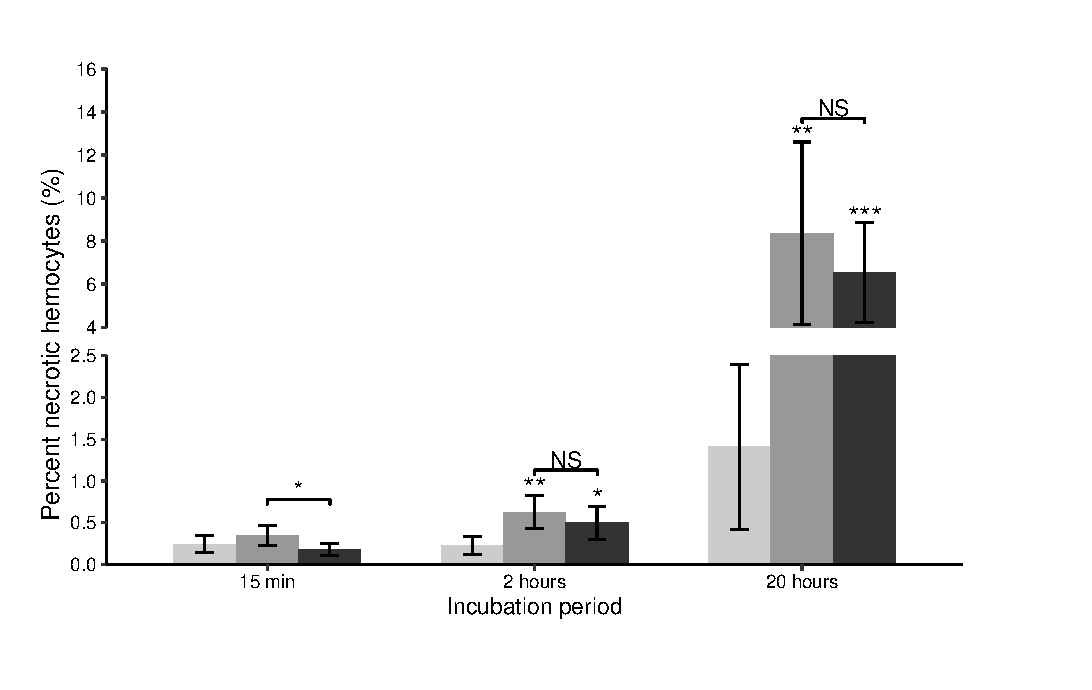
\includegraphics[width=1.13\textwidth]{figures/Method development/grouped bargraph scaled.pdf}
    \caption{The mean percentages of TO-PRO$^{TM}$-3 Iodide positive hemocytes after 15 minute, 2 hours and 20 hours incubation in \protect\lysegraabox \ Marine Physiological Saline Solution (n=8), \protect\customgraybox \ Anticoagulant Buffer (n=8) or \protect\darkgraybox \ Modified Alsever's Solution (n=8). Calcein acetoxymethyl (Invitrogen$^{TM}$) was used as a live cell counter-stain. Each datapoint is expressed as a percentage of 10.000 recorded hemocyte events, and the error bars represent 95\% confidence intervals of group means. Asterisks above error bars represent significance level of two sample t-test comparisons with }
    \label{fig:BufferViability}
\end{figure}

- Report results fro where I checked if EDTA changed the cytogram, because it would be nice to report that it doesn't affect them during the 15 minute incubation period.

MPSS = Marine Physiological Saline Solution aka. MPSS \cite{Hernroth2003}.
